\chapter{Implementation}

\begin{figure}[h]
	\centering
	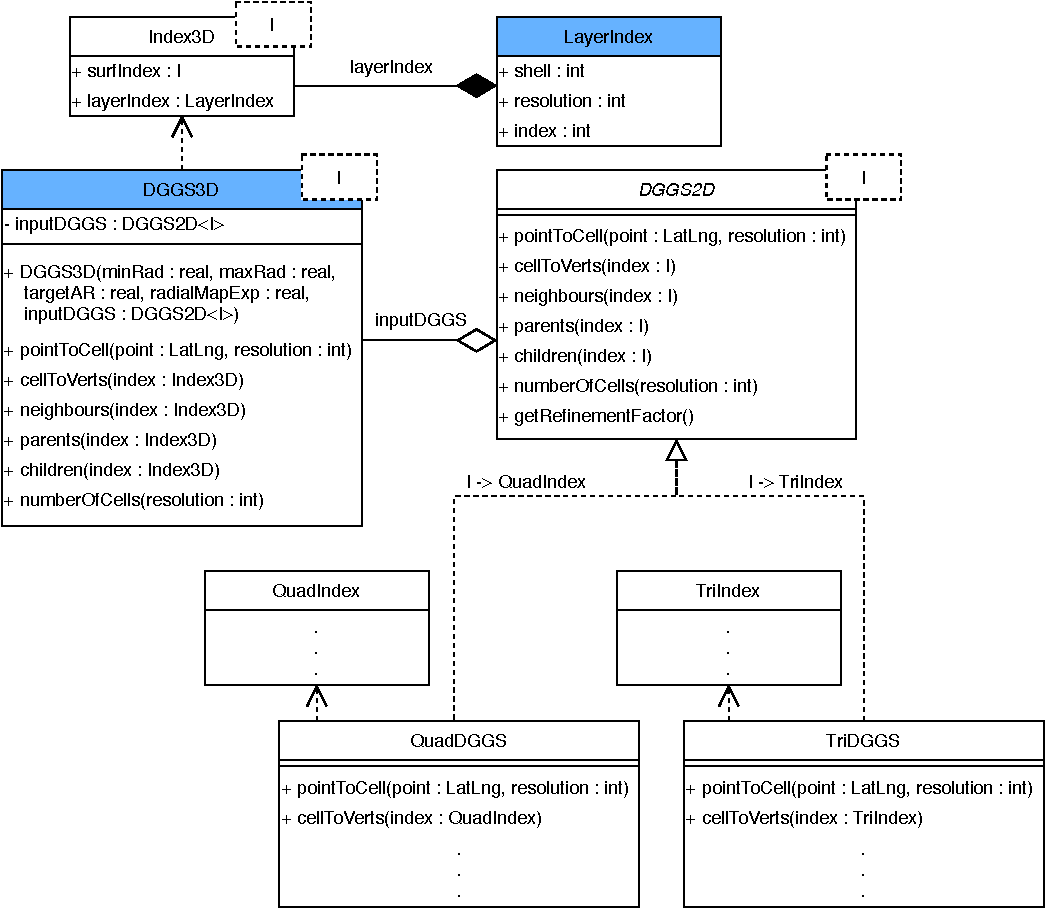
\includegraphics[width=\columnwidth]{3ddggs-uml.pdf}
	\caption{Class diagram for the implementation of our method. The classes shown in blue have their implementation and/or functionality described in the main body of the paper}
	\label{fig:uml}
\end{figure}

Figure~\ref{fig:uml} shows a class diagram for the C++ implementation of the grid extension method. \textit{DGGS2D} specifies the operations that must be provided by a conventional DGGS. It is an abstract class templated on a type to use as the index for the grid and specifies operations for encoding (pointToCell), decoding (cellToVerts), and standard indexing operations (neighbours, parents, and children). Additionally, it provides information regarding the number of cells in the grid at a given resolution (numberOfCells) and the factor of the employed refinement (getRefinementFactor). These are used by the 3D DGGS to obtain $n$ and $f$, respectively. QuadDGGS and TriDGGS are provided as two example DGGS2D implementations that could exist, which use QuadIndex and TriIndex as their index types, respectively.

During construction, a DGGS3D takes a reference to a \textit{DGGS2D} (the input DGGS) along with values minRad ($R_\mathrm{min}$), maxRad ($R_\mathrm{max}$), targetAR ($a$), and radialMapExp ($t$). This class is also templated on the type of the index used by the input DGGS. DGGS3D uses the class Index3D as its index type, which is simply a tuple composed of a surface index type and a LayerIndex. LayerIndex is a tuple of shell ($s$), resolution ($k$), and index ($j$).

For the implementation of encoding and decoding in the DGGS3D (pointToCell and cellToVerts), the radial mapping and layer parameterization steps described in Section~\ref{sec:encoding} are combined into single operations. For encoding, this means that LayerIndex is calculated directly from the radius without computing the actual value of $m(r)$. Likewise for decoding, the maximum and minimum radii ($r_\mathrm{min}$ and $r_\mathrm{max}$) are computed directly from $s$, $k$, and $j$ without first computing the values of $m(r_\mathrm{min})$ and $m(r_\mathrm{max})$. The separation of radial mapping and layer parameterization in Section~\ref{sec:encoding} is only done for conceptual clarity